\documentclass{article}
\usepackage{graphicx} % Required for inserting images
\usepackage[margin=3cm]{geometry}
\usepackage{biblatex}
\usepackage{hyperref}
\usepackage{cleveref}
\usepackage{listings}
\usepackage{tabularx}


\hypersetup{
    colorlinks=true,
    linkcolor=black,
    filecolor=magenta,      
    urlcolor=cyan,
    pdftitle={NEA (Route Planner)},
    pdfpagemode=FullScreen,
    }

\title{NEA \\Route Card and Route Planning tool}
\author{Jonty Beglin}
\date{April 2024}

\newcommand{\Q}{\bigskip\bfseries Q: }
\newcommand{\A}{\par\textbf{A:} \normalfont}

\newcommand{\Adv}{\bigskip\textbf{Advantages: }}
\newcommand{\Dis}{\bigskip\textbf{Disadvantages: }}

\newcommand{\QAnalysis}[4]{
    \noindent \textbf{Question #1: } #2 \\
    \noindent \textbf{Answer(s): } #3
    \begin{itemize}
        \item #4
    \end{itemize}
}

\newcommand{\InterviewQuestion}[3]{
    \noindent \textbf{Question #1: } #2 \\
    \noindent \textbf{Answer: } #3 \\
}

\newcommand{\testtable}[6]{
    \begin{center}
        \textbf{#1}
        \vspace{0.125cm}
        \vspace{0.25cm}
        \begin{tabularx}{\textwidth}{ |X|X|X|X| }
            \hline
            Testing & Objective & Pass/Fail & Notes \\
            \hline
            #2 & #3 & #4 & #5 \\
            \hline
        \end{tabularx}
        \\
        \vspace{0.25cm}
        \url{#6}
    \end{center}
}

\begin{document}

\maketitle

\newpage

\tableofcontents

\newpage


\section{Analysis}

    \subsection{The Problem}

        I would like to create a tool that allows users to plan hiking routes on an interactive UI featuring a map and waypoint capabilities. The tool should then be able to return to the user a route card that the user can use while on their hike to navigate along the path they have created within the program with useful information they may want such as bearings, walking times, distances and place names. An example of what could be displayed in the program can be seen in \cref{fig:example_map_dartmoor}.

        \begin{figure}[ht]
            \centering
            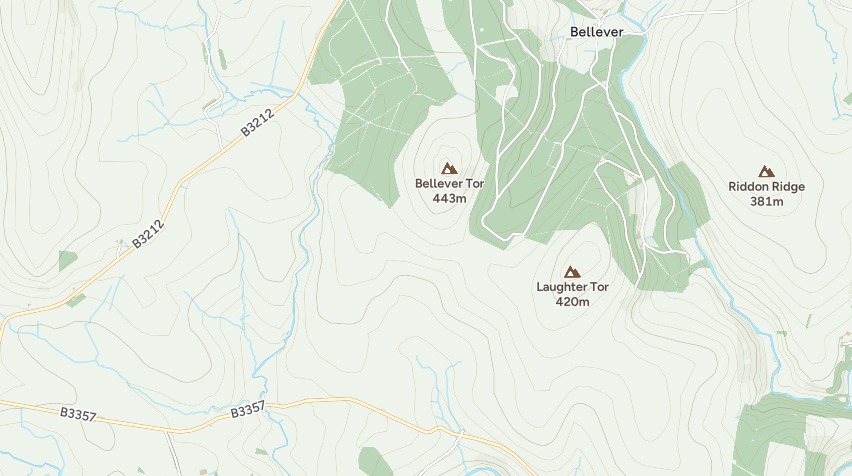
\includegraphics[width=0.75\textwidth]{Photos/Example/OSmapsExampleDartmoor.png}
            \caption{Example of a map which could be displayed within the program}
            \label{fig:example_map_dartmoor}
         \end{figure}

         Currently many people I know use pen and paper with physical maps to measure out distance and do manual calculations to create their route cards. I believe many people would benefit from this as it should be faster, easier and more accurate than traditional methods. I would further like to add options to load and save routes meaning users can edit their previously created routes.
         
         I would like to implement a feature to snap to paths to get more accurate readings of the path distance and time taken to walk a path. However, depending on which APIs are used and what data is available this may not be possible to achieve in some circumstances due to the disparity between the real world and the data online.
         
        \begin{figure}[ht]
            \centering
            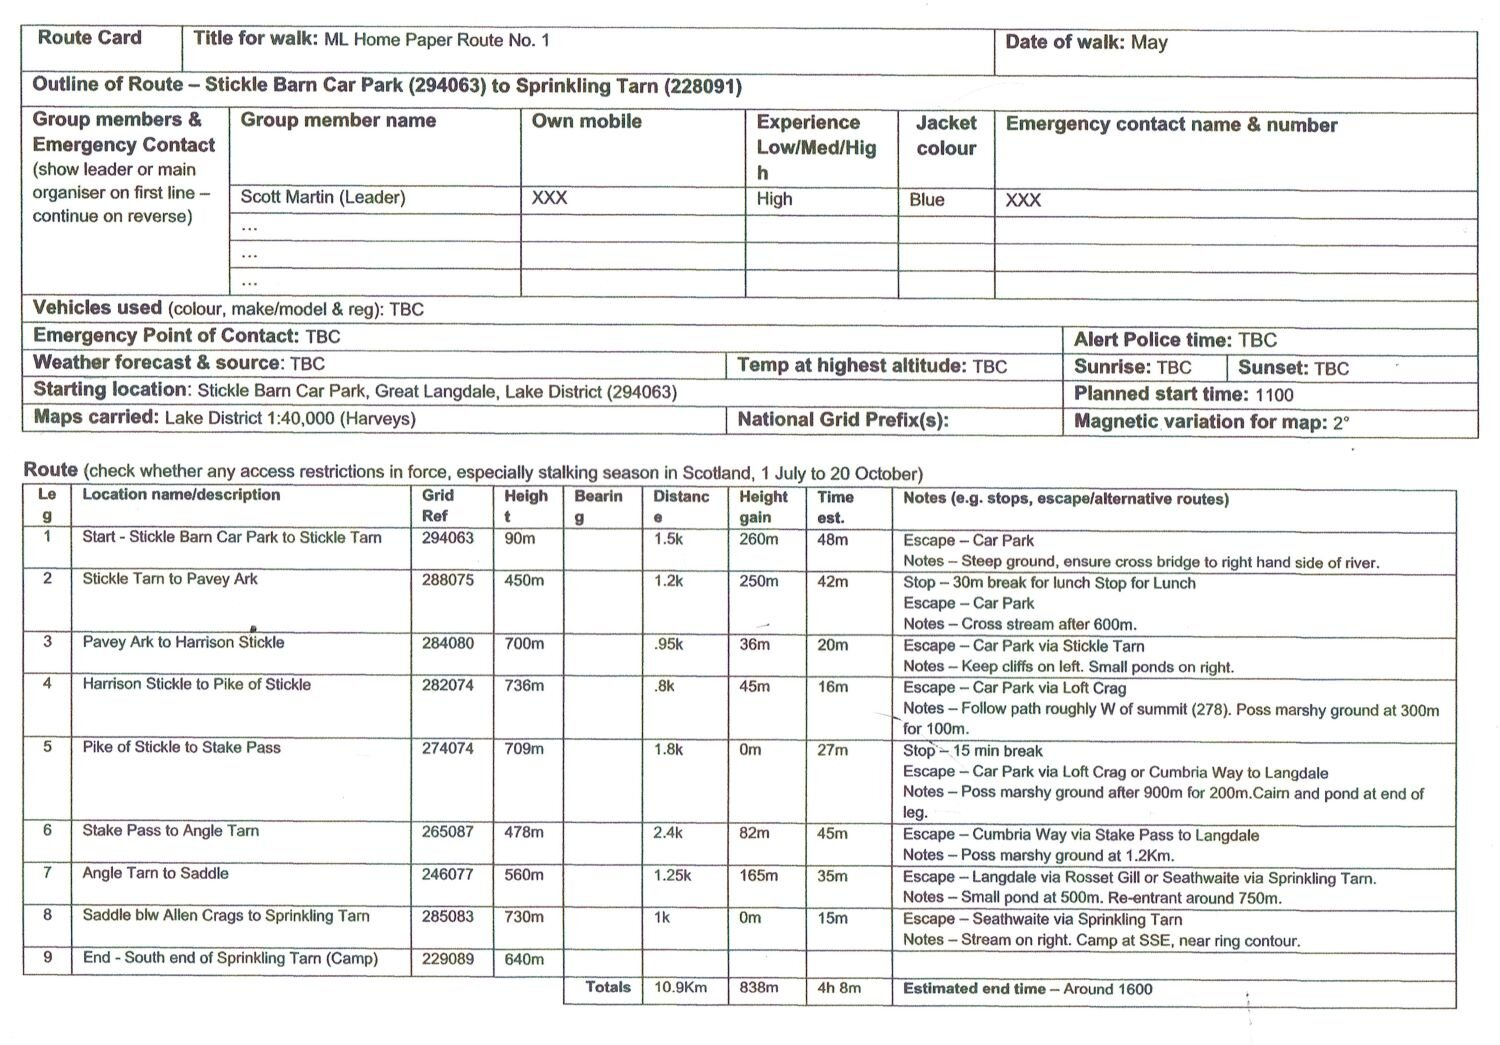
\includegraphics[width=0.75\textwidth]{Photos/Example/RouteCardExample.jpg}
            \caption{Example of a Route Card which could be generated from the program}
            \label{fig:example_route_card}
         \end{figure}
         
         I think there should be options for how the route card will be laid out, potentially allowing the user to directly edit the route card which will be outputted. This may be a sub-program within the main program which enables the user to view and edit the data of the route card. An example route card which the program should aim to output can be seen in \cref{fig:example_route_card}.

    \subsection{Mapping APIs}

        Choosing the most suitable API for gathering map data is paramount to the project's success. The map data needs to be able to be accessed relatively quickly and reliably, the user could potentially interact with an interactive map as seen in Google Maps and draw the route in real-time, however, this may be out of the scope of the project, so instead I could allow the user to use an interactive map to find a snapshot location of their "work area" where then they can draw their route on top of which will have an inbuilt scale automatically scaled to the same scale as when they were using the interactive map. The user's waypoint locations could be saved to allow for the later creation of a route card or as previously mentioned create a route which can be edited or expanded upon later. Optimally the mapping API should allow me to feed in some latitude and longitude and it feed back some mapping data in the form of a photo or other source which can then be overlaid onto the screen and I could use some module such as pygame or tkinter in python to move based on the user's actions.

        \subsubsection{Google Maps}

            The Google Maps API seems to be the most popular mapping API used by businesses and for some personal use. Upon the creation of a Google developer account and attempting to generate an API key I was prompted to input card details for future payment which is out of the question for this project, furthermore, I believe the Google Maps API is more suitable for businesses displaying their locations in a browser with Google Maps meaning users can more easily see where the business is located. I tried for a while to attempt to use the Google Maps map tiles API to get terrain tiles and satellite tiles both of which did not work as I could not successfully generate a session token. Here is the code I was using to attempt to generate a session token, replacing API\_KEY with my API key generated by Google as seen below. This in the end did not work and I couldn't change any of the google maps setting to be able to allow me to generate an API session key.

            \definecolor{codegreen}{rgb}{0,0.6,0}
            \definecolor{codegray}{rgb}{0.5,0.5,0.5}
            \definecolor{codepurple}{rgb}{0.58,0,0.82}
            \definecolor{backcolour}{rgb}{0.95,0.95,0.92}
        
            \lstdefinestyle{mystyle}{
                backgroundcolor=\color{backcolour},   
                commentstyle=\color{codegreen},
                keywordstyle=\color{magenta},
                numberstyle=\tiny\color{codegray},
                stringstyle=\color{codepurple},
                basicstyle=\ttfamily\footnotesize,
                breakatwhitespace=false,         
                breaklines=true,                 
                captionpos=b,                    
                keepspaces=true,                 
                numbers=left,                    
                numbersep=5pt,                  
                showspaces=false,                
                showstringspaces=false,
                showtabs=false,                  
                tabsize=2
            }
        
            \lstset{style=mystyle}
            
            \lstinputlisting[language=Python]{AnalysisCode/googlemaps.py}

        \subsubsection{here.com}

            The Here API gave me access to exactly what I needed, allowing me to generate satellite photos at a specific zoom level centred around a point. Here is an example API query: \\

            \noindent
            https://1.aerial.maps.ls.hereapi.com/maptile/2.1/maptile/newest/satellite.day/\{zoom\}/\{x\}/\{y\}/\{size\} \\ /png8?apiKey=\{key\_secret\} \\

            Where x, y and the longitude and latitude respectively, zoom is the zoom level of the requested time, this is a value between 0 and 20 and allows me to get appropriately sized times. The size attribute is the resolution of the desired image, this is limited to 512 by the API. key\_secret is the API key. I used some example code as well as programmed myself a program to zoom into a specific point on a map which allows the user to use the scroll wheel to zoom in and out of a pre-determined point as well as use the arrow keys to move the camera around the map. This could be improved in a later version to generate and look at more than one tile at a time which increases resolution. The program could generate all the tiles in view of the camera so there is no blank space. Culling could then be used to remove the tiles which can not be seen by the camera. Below is the code I used to produce the images seen in \cref{fig:here_output}.

            \definecolor{codegreen}{rgb}{0,0.6,0}
            \definecolor{codegray}{rgb}{0.5,0.5,0.5}
            \definecolor{codepurple}{rgb}{0.58,0,0.82}
            \definecolor{backcolour}{rgb}{0.95,0.95,0.92}
        
            \lstdefinestyle{mystyle}{
                backgroundcolor=\color{backcolour},   
                commentstyle=\color{codegreen},
                keywordstyle=\color{magenta},
                numberstyle=\tiny\color{codegray},
                stringstyle=\color{codepurple},
                basicstyle=\ttfamily\footnotesize,
                breakatwhitespace=false,         
                breaklines=true,                 
                captionpos=b,                    
                keepspaces=true,                 
                numbers=left,                    
                numbersep=5pt,                  
                showspaces=false,                
                showstringspaces=false,
                showtabs=false,                  
                tabsize=2
            }
        
            \lstset{style=mystyle}
            
            \lstinputlisting[language=Python]{AnalysisCode/here.py}

            \begin{figure}[ht]
                \centering
                \includegraphics[width=0.75\textwidth]{Photos/Analysis/hereOutput.png}
                \caption{Output of the program using the HERE API to generate map tiles in python and pygame}
                \label{fig:here_output}
             \end{figure}
    
             The major downside of this API is the limited API requests per month being 1000 making it virtually impossible to use for a program which may have to do 1000's of requests within a few hours depending on the user's use. Due to this, I will be exploring other options for API data.

        \subsubsection{TomTom}

            The TomTom API, although very similar to the here API, allows for 50,000 tile requests per day which should be far more than enough so long as the tile requests are fast, reliable and accurate this could be the API I use. Here is an example request from the API: \\

            \noindent
            https://api.tomtom.com/map/1/tile/sat/main/\{zoom\}/\{x\}/\{y\}.jpg?key=\{API\_KEY\} \\

            This request returns an image based on the zoom, x value and y value, the api\_key is also needed. I am somewhat unsure on how the x and y values work as it seems to split the grid up into many tiles depending on your zoom level and the x and y I believe picks the tile from a mapping of tiles which cover the entire globe. This does need to be explored further as in my testing below the map would often end up in the wrong location, however on the highest zoom level the longitude and latitude is correctly converted to x and y which can be used by the program and generate the correct API request. An output of the code below can be seen in \cref{fig:tomtom_output}
                
            \definecolor{codegreen}{rgb}{0,0.6,0}
            \definecolor{codegray}{rgb}{0.5,0.5,0.5}
            \definecolor{codepurple}{rgb}{0.58,0,0.82}
            \definecolor{backcolour}{rgb}{0.95,0.95,0.92}
        
            \lstdefinestyle{mystyle}{
                backgroundcolor=\color{backcolour},   
                commentstyle=\color{codegreen},
                keywordstyle=\color{magenta},
                numberstyle=\tiny\color{codegray},
                stringstyle=\color{codepurple},
                basicstyle=\ttfamily\footnotesize,
                breakatwhitespace=false,         
                breaklines=true,                 
                captionpos=b,                    
                keepspaces=true,                 
                numbers=left,                    
                numbersep=5pt,                  
                showspaces=false,                
                showstringspaces=false,
                showtabs=false,                  
                tabsize=2
            }
        
            \lstset{style=mystyle}
            
            \lstinputlisting[language=Python]{AnalysisCode/tomtom.py}
            
            \begin{figure}[ht]
                \centering
                \includegraphics[width=0.75\textwidth]{Photos/Analysis/tomtomOutput.png}
                \caption{Output of the program using the TomTom API to generate map tiles in python and pygame}
                \label{fig:tomtom_output}
            \end{figure}
    
        % \subsubsection{MapBox}

            

    \subsection{Route Cards}

        There are many different intricacies behind route cards, their format, and what users view as important or less important. One example of this is one of the key parts of a route card, the location. There are only 3 options for what could be in the location section of each leg. Many people believe you should only put the location you are going to on the route card, the other popular option is both where you have come from and where you are going to. A generally far less popular option is to have exclusively where you have come from.

        \subsubsection{Naismiths rule}
        \label{subsubsec:naismiths_rule}

            Naismiths rule is used to help hikers to plan their routes and allow suitable time for climbing up mountains or up elevation. It states to allow for 1 minute of extra time for every 10 metres of elevation. This, in reality, is rather inaccurate and within a program, we can calculate this additional time required far more accurately. For example, we can use Pythagoras on a triangle where the y is the elevation and the x is the horizontal distance. Doing so we can find the additional distance which someone is required to travel. We can then apply some editable multiplier to this distance which can be added to the total time required to cross a specific leg. This I believe is a far more accurate and adjustable way to implement time calculations based on height, an example of this can be seen in \cref{fig:inclined-distance}. 

            \begin{figure}[ht]
                \centering
                \includegraphics[width=0.75\linewidth]{Photos/Analysis/triangle.png}
                \caption{How distance could be calculated}
                \label{fig:inclined-distance}
            \end{figure}

        \subsubsection{Bearings}

            Bearings are considered unnecessary by many hikers, however, some people can't live without them, so I believe the program should have an option to either have them on or off within the route card. This, like many other features within the program, can be user-specific and be saved with either a specific login or on a specific computer. 

            To calculate the bearing, so long as the map is to scale on both the x and y axis, it should not be too hard as it should just be the angle from vertical between two points so we could use matrix dot multiplication to get an angle between a vertical line from one point on the route to the line made between that point and the next point on the route. This will always give us an acute angle so we then may need to check which quadrant the second point is in relative to the first and adjust the angle accordingly an example of this can be seen in \cref{fig:bearing-desmos}.

            \begin{figure}[ht]
                \centering
                \includegraphics[width=0.75\linewidth]{Photos/Analysis/bearing.png}
                \caption{Example of bearing between two points}
                \label{fig:bearing-desmos}
            \end{figure}

        \subsubsection{Additional calculation columns}

            Many hikers including some which I have interviewed see it as traditional or necessary to have additional columns which may be redundant if a program is making a route card. For example, the time taken to travel from A to B without taking into account elevation. This will not be used on a hike or a route and is ultimately useless, however, I believe some people would see it as improper if it was left out. So as a result of this, I will aim to make a setting to change this such that its visibility can be toggled on and off.

    \subsection{User's Needs}

        \subsubsection{Questionnaire}

            My first method of analysing the user's need is through the use of a questionnaire sent out to the members of a local scout group to receive feedback on how they would want a program like this to functions and what features are the most important to the user. I also asked for any additional feedback which they could not provide through the previous fields. \\
            
            \QAnalysis{1}{How likely would you be to use a computer program to plan your route?}{Very likely, Somewhat likely, neither likely nor unlikely, Somewhat unlikely, Very unlikely}{Asking this question allows me to take into account how much a particular response should affect the way I plan my project. If a potential user is very unlikely to use a computer program to plan their route, I should not focus on tailoring the program to them.}

            \QAnalysis{2}{Which Features would you say are most important to you within the mapping tool?}{Accurate map information with paths on, Easy to use, Being able to move and edit points on the route, Route automatically going along a path, Saving routes}{This question allowed the user to order which features are the most important to them and thus allow me to build an ordered list of priority features which the end user would like to see the most.}

            \QAnalysis{3}{What features about the route card creator are most important to you?}{Automatically fills timings, Being able to edit the route card after creation, Automatically calculates elevation, Automatically calculates bearings, Automatically filled in emergency information}{Similar to the previous question, this allowed the user to order what features are the most important to them within the program but specifically within the route card editor/creator part of the program which highlights the important parts of the route card creator.}

            \QAnalysis{4}{How would you like the route card to be output to you so you can edit it if needed?}{Excel Spreadsheet, PDF, Within the program, Other: specify}{This gives me information about how the users may want the program to output the final route card to them. Creating a route card editor within the program may be hard and potentially less user-friendly, pdf would necessitate research into creating a pdf with adequate formatting.}

            \QAnalysis{5}{What information about each leg do you want?}{From (e.g. From Brentor), To (e.g. To Pewtor), From and To (e.g. From Brentor to Pewtor)}{This question truly dials into how the program should output route cards and what information should be given on on them and what would be most useful the end users.}

            \QAnalysis{6}{If you could have a login to the tool what features would you use (multiple choice)?}{Saving Routes, Saving Safety information (escape notes), Emergency contacts automatically filled in, Saving your typical walking speed, Sharing routes with others}{This was a multiple choice question which allowed users to select multiple of the proposed features allowing me to gauge which are the most important to the most users.}

            \QAnalysis{7}{How do you make your route cards (e.g. paper or online tools)?}{Text Box}{This question is to give me an insight into alternatives allowing me to research them and what their advantages and disadvantages may be so that I can take the pros and cons of each of them and attempt to make an overall superior program.}

            \QAnalysis{8}{Any other comments:}{Text Box}{This allows the respondent to add any additional information or opinions which were not captured by the previous questions.}

        \subsubsection{Interview}

            To gain an insight into my user's needs and wants for this project and how a typical user may want the program to function I interviewed a local scout group leader who could give me an insight into what general users (scouts) of the program may be looking for or features they may find useful. I found this very useful in making choices about the program and this gave me some additional ideas I hadn't yet thought about. \\

            \InterviewQuestion{1}{Would your scout group actually get use of mapping features outside of Dartmoor and if so would it be worth a reduction in features in Dartmoor?}{Most of our activities are local to Tavistock within the Dartmoor area.}

            \InterviewQuestion{2}{Do you want to be able to click on points of interest such as Tors so that waypoints snap to points of interest?}{Yes that would be very useful as we go to Tors and points of interest often on our walks.}

            \InterviewQuestion{3}{Would you prefer to draw routes onto the map using the cursor and a waypoint system or being able to choose and put together pre-made routes between points of interest with more accurate distances?}{Definitely using the cursor and waypoints as I need the group to stay on the correct path which they have planned out.}

            \InterviewQuestion{4}{Do you want to be able to see contour lines on the map while you are planning your route?}{Yes.}

            \InterviewQuestion{5}{Would you want the program to automatically integrate the height and elevation of the route into the timing calculations}{Yes it would be very useful, however, I would like the option to turn it off so I can get the scouts to fill it in by hand.}

            \InterviewQuestion{6}{How important are features such as zooming, undoing as well as saving a route, is there any other features which would be important to you?}{Zooming is not so important as long as I can accurately see the route I am plotting, Undo is hugely important as I often change my mind while planning a route. Saving would be incredibly useful to share the route with others. Being able to easily move the map around and edit different parts of the route is very important as well.}

            \InterviewQuestion{7}{Would you want to be able to name waypoints to help automatically fill out the created route cards}{Not important.}

            \InterviewQuestion{8}{Once you've finished editing would you want to see the waypoints or just the route?}{Having the waypoints could be useful.}

            \InterviewQuestion{9}{When you're mapping do you want to add each leg or decide the legs at the end of creating the route?}{I'd like to do it in sections so that I can edit each leg individually.}

            \InterviewQuestion{10}{Because the timings and elevations are calculated automatically, some columns on the route card could be made redundant, e.g. time without elevation. Would any of your scout members benefit from seeing these columns anyway?}{It would be really useful to be able to have them on or off based on a setting before the route card is printed.}

            \InterviewQuestion{11}{When you calculate timings for elevation would you like to go with the standard Naismiths rule seen in \cref{subsubsec:naismiths_rule} or more advanced calculations such as taking into account the walking speed and extra distance travelled due to elevation?}{The more customisable the better, I would like to edit the time taken to go uphill be it could be an option.}

            \InterviewQuestion{12}{How would you like the program to output the route card to users?}{No real preference as long as I can print it out.}

            \InterviewQuestion{13}{Would you find a login to the program useful, what information would you want saved with it?}{A login would be very useful. I would want it to remember my previous options I have set and save emergency contacts and the people on the walk and walking speed options.}

        \subsubsection{What I learnt}
        
            Overall I found the interview and questionnaire very helpful and I will try to build my final product as close to this specification as possible. I hadn't realised the importance of an undo feature and misjudged the importance of waypoints. It would seem the key details of the program are that the user can draw accurate routes which they will follow on the route, this includes having accurate distances and timings which can be output to a route card. Additionally, I hadn't considered the program being used primarily as an educational tool for scouts. Interviewing a scout leader highlighted the potential for the tool to be used by younger people to teach them about route planning and even aid in teaching the calculations necessary to create a route card. Here are some of the main takeaways from both the interview and questionnaire combined:

            \begin{itemize}
                \item Most people would not benefit from the program working outside of the Dartmoor area.
                \item Ease of use and features such as snapping to points of interest are very important to many users so this should be a main objective.
                \item Being able to accurately plan routes is essential, so having up-to-date map data and an accurate route planner are vital.
                \item Although the route card information automatically being filled in is very useful (such as timings and elevations), a scout leader may want to turn this setting off to allow scouts to fill the information in themselves as an educational tool.
                \item An undo button is essential, this would also indicate that there should be an easy way to edit specific parts of the route, for example between two points within the route there should be some way to edit the middle part.
                \item Although I believed zooming to be vital in the project, it turns out that the scout leader did not view it as a vital feature. 
                \item A waypoint naming system is not important and instead I will design the program such that each leg of the route will be edited individually and named accordingly.
                \item Making settings such as walking speed and additional height calculations should be made as customisable as possible as each individual user has their own changes and needs they would want within the program.
                \item Many users wanted the route card to be output within the program however I believe as long as the output can either be printed or easily copied or transferred to another medium users will be happy with the results.
                \item Many users would find use in a login, primarily so that they can share routes, edit them later or reuse routes.
            \end{itemize}

    \subsection{Existing solutions}

        \subsubsection{Pen and paper}

            Using pen and paper garnered 6 out of the 12 responses, which is surprising as I believed this number would be far higher. Using pen and paper entails using a physical map, ruler, pencil and rubber to plan a route and then also transfer it to a physical route card drawing the rows and columns out.

            \Adv
            \begin{itemize}
                \item Users can see contour lines to aid them plan their route.
                \item Users can lay out their route cards how they want.
                \item Easy to edit the route on pen and paper as lines can be erased whenever the user wants.
                \item No learning curve and easy to understand.
            \end{itemize}

            \Dis
            \begin{itemize}
                \item Older maps may be out of date and thus incorrect.
                \item Creating a route card would be very time-consuming.
                \item Calculations may be incorrect when working with many numbers.
                \item The user may not possess the physical map to go on the hike they want.
                \item Cannot be edited easily after creation.
                \item Hard to change values such as walking speed or elevation calculations.
            \end{itemize}

        \subsubsection{Excel}

            Another popular option for other tools people use while creating their route cards and routes is through the use of a map, sometimes in an online form such as Google Maps. And Excel to create the route card itself with a predetermined template. An example route card can be seen in \cref{fig:route-front} and \cref{fig:route-back}.

            \begin{figure}[ht]
                \centering
                \includegraphics[width=0.75\linewidth]{Photos/Analysis/routeCardFront.jpg}
                \caption{Front of an example route card in excel}
                \label{fig:route-front}
            \end{figure}

            \begin{figure}[ht]
                \centering
                \includegraphics[width=0.75\linewidth]{Photos/Analysis/routeCardBack.png}
                \caption{Back of an example route card in excel}
                \label{fig:route-back}
            \end{figure}
            
            \Adv
            \begin{itemize}
                \item Calculations can be performed automatically reducing human error and saving time.
                \item Users can modify the template to their liking and specific needs.
                \item Excel files can easily be saved and shared.
            \end{itemize}

            \Dis
            \begin{itemize}
                \item May have a steep learning curve for some users.
                \item Still requires manual input.
                \item Users must refer to an external mapping tool
                \item May be prone to data input errors.
            \end{itemize}

        \subsubsection{OS maps}

            OS maps is an online program which can be used to plan routes using a waypoint system. A number of my questionnaire respondents mentioned it as a tool that they use. One primary drawback of this tool is that it does not generate route cards automatically for you after planning your route, thus still leaving all the disadvantages of either Excel or pen and paper. An example route from OS maps can be seen in \cref{fig:os-maps-example}

            \begin{figure}[ht]
                \centering
                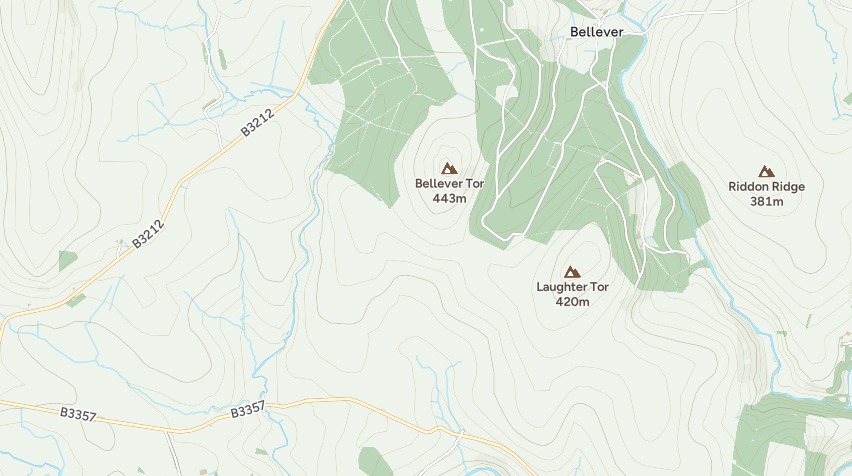
\includegraphics[width=0.75\linewidth]{Photos/Example/OSmapsExampleDartmoor.png}
                \caption{Example route in OS maps}
                \label{fig:os-maps-example}
            \end{figure}

            \Adv
            \begin{itemize}
                \item 
            \end{itemize}

            \Dis
            \begin{itemize}
                \item 
            \end{itemize}
        
\newpage

\section{Documented Design}

    

\newpage
    
\section{Technical Solution}

    

\newpage

\section{Testing}

    

\newpage

\section{Evaluation}

    
    
\end{document}
